% !Mode:: "TeX::UTF-8"

\documentclass{svk_short_sk}
%% ak pisete po anglicky, pouzijete namiesto horneho riadku
%% \documentclass{svk_short_en}

\newenvironment{nscenter}
 {\parskip=0pt\par\nopagebreak\centering}
 {\par\noindent\ignorespacesafterend}

\begin{document}
\title{Inov\'acia prostredia Karel 3D a jeho vyu\v{z}itie vo vyu\v{c}ovan\'i}

\author{Tom\'a\v{s} Kubla\inst{1}
\email{kubla1@uniba.sk}
}
%% vsimnite si, ze u autorov sa nepisu tituly
%% prikaz \inst sluzi ako odkaz do zoznamu institucii
%% (vid. nizsie)

%% skolitela nepiste medzi autorov, ale v tejto casti
%% ak praca nema skolitela, jednoducho vynechajte
\supervisor{Monika Tomcs\'anyiov\'a\inst{2}
\email{tomcsanyiova@fmph.uniba.sk}}

%% nasleduje kratka verzia nazvu clanku a 
%% zoznam autorov (bez krstnych mien)
%% tieto informacie sa zobrazuju v hlavicke
\titlerunning{Inov\'acia prostredia Karel 3D a jeho vyu\v{z}itie vo vyu\v{c}ovan\'i}
\authorrunning{Kubla}

\institute{
Katedra informatiky,
FMFI UK,
Mlynská Dolina,
842~48,~Bratislava
\and
Katedra základov a vyučovania informatiky,
FMFI UK,
Mlynská Dolina,
842~48,~Bratislava}

\maketitle

Školský predmet informatika sa na Slo\-ven\-sku vyučuje na oboch stupňoch ZŠ.
Jej ciele, obsah a rozsah sú určené v dokumente \cite{SPU}.
Pre tematický okruh \emph{Algoritmické riešenie problémov} na 2. stupni ZŠ sa v dokumente píše, aby žiaci pracovali v nejakom programovacom prostredí.
Je dobré, ak má učiteľ k dispozícii niekoľko alternatív programovacích prostredí, ako napr. \emph{IzyLogo}, \emph{Panák} alebo \emph{Karel}.

Prostredie Karel 3D \cite{KOSUT97} používali učitelia na Gymnáziu Jura Hronca, a podľa ich ohlasov bolo pre žiakov atraktívne, s intuitívnym ovládaním.
Keďže išlo o open-source program, rozhodol som sa využiť možnosť rozšíriť ho o niekoľko nových možností.
Mojím prínosom bolo:
preklopenie programu z prostredia Delphi do Lazarusu;
oprava niekoľkých chýb, ktoré boli zistené používateľmi;
pridanie možnosti vytvárania zadaní učiteľom tak, aby sa stali súčasťou samotného prostredia;
vytvorenie ladiaceho prostredia;
príprava metodiky na vyučovanie s cieľom venovať sa predovšetkým metodike vyučovania rekurzie pre žiakov, ktorí majú záujem o programovanie.

Novým prvkom mojej implementácie je možnosť pridávania zadaní úloh učiteľom priamo v prostredí Karel 3D.
Za zadanie sa považuje sada malých či väčších úloh, ktoré majú počiatočný stav miestnosti a pozície postavičky Karla (do ktorej sa vie používateľ počas riešenia vrátiť), slovný popis a vizuálnu ukážku správneho riešenia, ktorá je dôležitá na to, aby žiak rýchlo pochopil, ako má vyzerať výsledný stav miestnosti po vyriešení zadanej úlohy.

Jednou z úloh ladiaceho nástroja v programovacích prostrediach je, že žiak má možnosť v prípade nefunkčného resp. nesprávne fungujúceho programu krokovať svoje riešenie a sledovať stav premenných, a podmienok.
Ďalším prínosom ladenia je, že žiak môže krokovať a analyzovať cudzie programy, čo učiteľovi umožňuje definovať priamočiaro ciele vyučovania informatiky aj pre štvrtý stupeň Bloomovej taxonómie (analýza).

Metodika, ktorú som pre prostredie vytvoril obsahuje môj návrh postupnosti tém, t.j. v akom poradí majú žiaci preberať jednotlivé programátorské konštrukcie jazyka Karel 3D.
K metodike sú pripravené ukážkové úlohy, a tiež cvičenia, ktoré kombinujú jednotlivé koncepty.

Za jej najväčší prínos považujem návrh postupnosti príkladov a úloh, ktoré umožňujú žiakov na~2.~stupni naučiť princíp rekurzie.
Tento prístup je založený na tom, že ak žiaci riešia jednoduché úlohy, dokážu im porozumieť a sú schopní pochopiť princípy rekurzie.
Dokument \cite{SPU} princíp rekurzie nevyžaduje, ja ho však odporúčam zaradiť do vyučovania pre šikovných žiakov.
 
\begin{nscenter} 
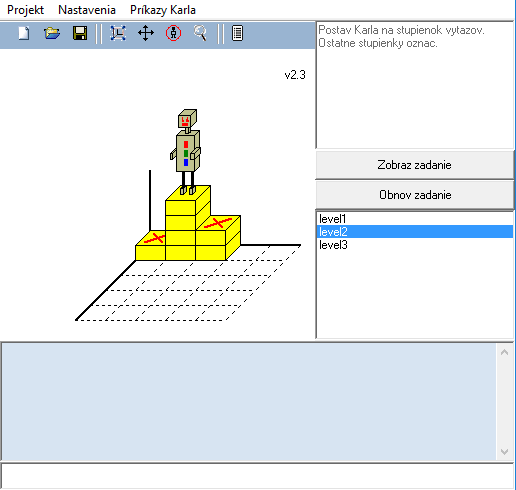
\includegraphics[width=0.266\textwidth]{images/karelNaStupni}
\end{nscenter} 

Prostredie Karel 3D, ktoré som rozšíril o nové možnosti, ponúka učiteľovi a jeho žiakom na~2.~stupni ZŠ, alternatívny programovací jazyk.
Vďaka mojej práci má učiteľ k dispozícii metodiku vyučovania a možnosť pridávania úloh priamo v prostredí.
Žiaci ním získali možnosť ladenia programu a vizualizácie riešenia.
Verím, že učiteľ a aj jeho žiaci tak získali ďalšie programovacie prostredie, v ktorom sa môžu učiť koncepty stanovené v iŠVP pre oblasť Algoritmické riešenie problémov.


\bibliographystyle{apalike}
\bibliography{literatura}

%% citacie ulozte do suboru references.bib
%% na populaciu zoznamu literatury pouzite program
%%
%% bibtex references
%%
%% po ktorom je potrebne dokument znova zlatexovat

\end{document}
